
\documentclass[10pt,a4paper]{report} 
%\usepackage{showkeys}
%\usepackage[left=3.5cm,right=2cm,top=2cm,bottom=2cm]{geometry}
\usepackage[top=0.70in, bottom=0.70in, left=0.8in,right=0.80in]{geometry}

%\usepackage[compact]{titlesec} % used to adjust space between
\usepackage{titlesec}                               % chapter title and text                               
\usepackage{etex}      
\usepackage{color}                          
\usepackage{setspace}
\usepackage{amsmath}
\usepackage{amsfonts}
\usepackage{amssymb}
\usepackage{array}
\usepackage{algorithmic}
\usepackage{algorithm2e}
\usepackage{layout}
\usepackage{url}
\usepackage{cite}
\usepackage{color}
\usepackage[standard,thmmarks,amsmath,hyperref]{ntheorem}
%\usepackage[implicit=false]{hyperref}
%\usepackage{etex}
\usepackage{graphicx}
\usepackage[nottoc]{tocbibind}%
%\usepackage{pgf}
\usepackage{times}
\usepackage{comment}
%\usepackage{booktabs}
%\usepackage{longtable}
\usepackage{alltt}
 \usepackage{fancyhdr}
 
 \usepackage[utf8]{inputenc}
 %\usepackage{mathptmx}
%\renewtheorem{definition}{Definition}[chapter]


\titleformat{\chapter}{\normalfont\huge\centering}{\Huge \bf  \thechapter.}{14pt}{\Huge \bf } %This is here, so that at each chapter start, I only get "chapter number + chapter name"

\begin{document}
\onehalfspacing



%\begin{comment}
\begin{titlepage}

\newcommand{\HRule}{\rule{\linewidth}{0.5mm}} % Defines a new command for the horizontal lines, change thickness here


\center % Center everything on the page
 
%----------------------------------------------------------------------------------------
%	HEADING SECTIONS
%----------------------------------------------------------------------------------------

{\Large \bfseries A}\\[0.45cm] %

{ \Large \bfseries PROJECT REPORT }\\[0.30cm] % Title of your document
%\vspace{0.5in}
{ \Large \bfseries on}\\[0.45cm]
{ \LARGE \bfseries SPAM DETECTION AND SENTIMENT ANALYSIS}\\[0.55cm]
\vspace{0.25in}
{ \Large \bfseries Submitted in partial fulfillment for the Award of Degree of}\\[0.35cm]
{ \Large \bfseries BATCHELOR OF ENGINEERING}\\[0.35cm]
{\Large IN}\\[0.35cm]
{ \Large \bfseries INFORMATION TECHNOLOGY}\\[0.35cm]
{\Large BY}\\[0.3cm]
{ \large \bfseries Divyanshu Alok (160116737122)}\\[0.1cm]
{ \large \bfseries Don Richardson (160115737095)}\\[1cm]
%----------------------------------------------------------------------------------------
%	AUTHOR SECTION
%----------------------------------------------------------------------------------------

\center
{\Large Under the guidance of}\\[0.3cm]
{\Large \bfseries Mrs. Trupthi M.}\\
{\Large Asst. Professor,}\\
{\Large Dept. of IT, CBIT}\\
\vspace{0.35in}


% If you don't want a supervisor, uncomment the two lines below and remove the section above
%\Large \emph{Author:}\\
%John \textsc{Smith}\\[3cm] % Your name

%----------------------------------------------------------------------------------------
%	DATE SECTION
%----------------------------------------------------------------------------------------
% Date, change the \today to a set date if you want to be precise

%----------------------------------------------------------------------------------------
%	LOGO SECTION
%----------------------------------------------------------------------------------------

 % Include a department/university logo - this will require the graphicx package

\includegraphics [width=40 mm]{cbit.png}\\
\vspace{0.35in}

\textsc{\Large \bfseries DEPARTMENT OF INFORMATION TECHNOLOGY}\\[0.5mm]
\textsc{\Large \bfseries CHAITANYA BHARATHI INSTITUTE OF TECHNOLOGY (A)}\\[0.5mm]
\large \bfseries{(Affiliated to Osmania University; Accredited by NBA (AICTE) and NAAC (UGC), ISO}\\
\large\bfseries{Certified 9001:2015), GANDIPET, HYDERABAD – 500 075}\\
Website:www.cbit.ac.in\\
2018-2019
%----------------------------------------------------------------------------------------
\vfill
% Fill the rest of the page with whitespace

\end{titlepage}
\pagenumbering{roman}
%\layout
 \allowdisplaybreaks
\vspace{0.5cm}
\begin{center}
	\textsc{\Large \bfseries CHAITANYA BHARATHI INSTITUTE OF TECHNOLOGY (A)}\\[0.3cm]
\textsc{\Large \bfseries DEPARTMENT OF INFORMATION TECHNOLOGY}\\[0.3cm]
\text{\bfseries(Affiliated to Osmania university)}\\[0.3cm]
\text{\large \bfseries GANDIPET, HYDERABAD – 500075}\\[1.5cm]

\includegraphics [width=40 mm]{cbit.png}\\[1.5cm]
\end{center}\

\centerline{\Large \bfseries CERTIFICATE}
\addcontentsline{toc}{chapter}{Certificate}
\vspace{0.5in}
\large{
This is to certify that the project work entitled \textbf{“Spam Detection and Sentiment Analysis”} submitted by \textbf{Divyanshu Alok} (160116737122) and \textbf{Don Richardson} (160115737095) in partial fulfilment of the requirements for the award of the degree of \textbf{BACHELOR OF ENGINEERING} in \textbf{INFORMATION TECHNOLOGY} to \textbf{CHAITANYA BHARATHI INSTITUTE OF TECHNOLOGY(A)}, affiliated to \textbf{OSMANIA UNIVERSITY}, Hyderabad, is a record of bonafide work carried out by them under my supervision and guidance. The results embodied in this report have not been submitted to any other University for the award of any other Degree or Diploma.

\vspace{1.5in}
\bfseries
\noindent PROJECT GUIDE \hfill HEAD OF DEPARTMENT \\
\noindent \normalfont \textbf{ Mrs. Trupthi M } \hfill \textbf{Dr. Suresh Pabboju}\\
\noindent \normalfont Asst. Professer,\hfill \normalfont Head of Department\\
\noindent \normalfont Dept of IT.\hfill \normalfont Information Technology\\
\noindent \null \hfill \normalfont CBIT , Hyderabad



\vspace{1in}

\vspace{1.5in}
% 
% \begin{center}
% Dean \\
% School of Mathematics and Computer / Information Sciences \\
% University of Hyderabad \\
% Hyderabad
% \end{center}
}
\newpage

\centerline{\LARGE \bfseries  Acknowledgement}
\addcontentsline{toc}{chapter}{Acknowledgements}
\vspace{0.5in}

\large{
It is our privilege to acknowledge with deep sense of gratitude and devotion for keen personal interest and invaluable guidance rendered by our Project Guide   Mrs. B Veera jyothi, Assistant Professor, Department of IT, Chaitanya Bharathi Institute of Technology.

\vspace{0.5cm}

We take the opportunity to express our thanks to \textbf{Dr. Suresh Pabboju} , Professor and Head of IT Department, CBIT for his valuable suggestions and moral support.

\vspace{0.5cm}


We are grateful to our Principal \textbf{Dr. P Ravinder Reddy}, Chaitanya Bharati Institute of Technology, for his cooperation and encouragement. 

\vspace{0.5cm}

Finally, we also thank all the staff members, faculty of Dept. of IT, CBIT, and our friends, who with their valuable suggestions and support, directly or indirectly helped us in completing this project work


\vspace{0.5cm} 
}
\newpage
\centerline{\LARGE \bfseries Declaration}
\addcontentsline{toc}{chapter}{Declaration}
\vspace{0.5in}

We declare that the project report entitled \textbf{“Parent Pal”} (an android project) is being submitted by me in the Department of Information Technology, Chaitanya Bharathi Institute of Technology, Osmania University.\\ \\
This is record of bonafide work carried out by me under the guidance and supervision of Mrs. B Veera Jyothi, Assistant Professors, Dept of IT, C.B.I.T.\\ \\
No part of the thesis copied from books/journals/internet and wherever the portion is taken, the same has been duly referred in the text. The reported are based on the project work doing entirely by me and not copied from any other source.




\vspace{0.6in}

\begin{flushright}
Divyanshu\\
160116737122\\
Don Richardson\\
160115737095\\
\end{flushright}


\newpage


\centerline{\LARGE \bfseries Abstract}
\vspace{0.25in}
\addcontentsline{toc}{chapter}{Abstract}

\medskip
Technology can be a little more disadvantageous than it is advantageous if it is not used by the right
people, in the right time for the right period. In this generation-X, toddlers are way more fluent with
gadgets than many people are. As positive as it may seem on one end, this might kill the creativity
and the colour of social relationship in a kid’s life. Usage of mobile phones and other electronic
gadgets among kids has to be controlled.

\vspace{0.25in}

In an attempt to solve this problem statement this application called “Parent-Pal“ is
developed. This application will provide information of various apps usage in a child’s gadget to the
parent/guardian. The application gets the information of the battery used on different applications
from the phone and with that information, calculates the time spent on each application. This is how
the application works on the child’s end. This information is taken into the database and is stored
there. This data is sent to the parent end of the application for the parent to monitor the usage of
the different applications on the child’s phone. This can also be used in offices to help supervisors in
monitoring the usage of the phone provided by the office to its employees. This application attempts
to give us the control over the technology that we invented. The parent or the manager can hide
this application from the child/employee on their phone. 

\vspace{0.25in}

This application will be built on React-Native using JavaScript. As it is built on React-Native,
this app will be a cross-platform application i.e. it can be used on both android and iOS devices.

\vspace{0.5in}
\begin{flushleft}
\noindent Tools used:\\
React-native\\
Android Studio\\
Firebase\\
Sublime text (text editor)\\
\end{flushleft}
\begin{flushright}
\noindent Submitted by: \\
\noindent Divyanshu(160116737122)\\
\noindent Don Richardson(160115737095)\\
\end{flushright}

\vfill
\newpage




 \tableofcontents
 \listoffigures

\clearpage
\onehalfspacing      % one and half line spacing 
%\doublespacing
\pagenumbering{arabic}

 \chapter{INTRODUCTION}
 
\section{Motivation}
In this digital era where most of us really busy all the time that parents (or a guardian) somehow loose track of their children , of their whereabouts and what are their interests.monitoring interests is a really important asset for nurturing a child and also making sure that this digital era does not affect them much. To help people with the mentioned problem we came up with a hybrid app (android and ios) and basically shares and battery use information between devices by making use of native modules.

\section{Existing system}
Presently there is no organised system to do so. Only thing guardians used to do and have doing is just checking their phone on random moments or just asking them
  
\pagenumbering{arabic}
\section{Objective of the project}
Objective is to establish a communication like a simple sender/receiver function between two ends namely a parent and a child. The data being communicated is gathered by flaunting the battery use information technically mentioned as intent.ACTION\_POWER\_USAGE\_SUMMARY . Communicating this lead to the parent knowing the amount of time spent on an application as power used by a particular application is roughly proportional to time spent on it.

\section{Tools and technologies used}
Tools needed for the successful execution of application:
\begin{itemize}
	\item Android device running on android 6 (Android Marshmallow) or latest
	\item Working internet connection
\end{itemize}
\vspace{3cm}
Technologies required for the successful build up of the application: 
\begin{itemize}
	\item React-native
	\item Android Studio (AVD)
	\item Sublime text 3 (text editor)
	\item Firebase (database)
\end{itemize}

\section{Organisation of report}
The organisation of the report is as follows:\\\\
\textbf{Chapter 1} deals the introduction part of the project.\\
\textbf{Chapter 2} deals with the technologies used for building the project.\\
\textbf{Chapter 3} deals with the software requirements while building the project.\\
\textbf{Chapter 4} shows the system design.\\
\textbf{Chapter 5} contains implementation.\\
\textbf{Chapter 6} shows result of the project.\\
\textbf{Chapter 6} explains the conclusion and future scope.\\
\newpage
%\end{comment}
\chapter{TECHNOLOGIES USED}
\section{React-native}
\subsection{About}
React Native is the next generation of React - a JavaScript code library developed by Facebook and Instagram, which was released on Github in 2013. Native app creation simply means writing apps for a specific operating system. React Native helps developers reuse code across the web and on mobile. React Native lets you build mobile apps using only JavaScript. It uses the same design as React, letting you compose a rich mobile UI from declarative components.With React Native, you don’t build a "mobile web app”, an "HTML5S app", or a “hybrid app”. You build a real mobile app that’s indistinguishable from an app built using Objective-C or Java. React Native uses the same fundamen- tal UI building blocks as regular iOS and Android apps. You just put those building blocks together using JavaScript and React.

\subsection{Advantages of React-native}
React Native lets you build your app faster. Instead of recompiling, you can reload your app instantly. With Hot Reloading, you can even run new code while retaining your application state.
React Native combines smoothly with components written in Objective-C, Java, or Swift. It’s simple to drop downto native code if you need to optimize a few aspects of your application. It’s also easy to build part of your app in React Native, and part of your app using native code directly - that’s how the Facebook app works.
The biggest difference is that its cross platform i.e engineers won’t have to build the same app for iOS and for Android from scratch, they can reusing the code across each operating system.

\subsubsection{Still Improving}
React Native isn’t perfect, in fact, it does have some clear limitations.
Some custom modules are missing, meaning that you might lose out on some of its time-saving perks but having to build and create your own.
\vspace{3cm}

\subsubsection{Still technical}
It’s easy to get swept up in React Native’s pre-packaged elements. However, for certain things, you'll still need a developer at hand to take care of some technical nasties.
These include incorporating smartphone camera accessibility into an app or push notifications and more sophisticated data handling.

\subsubsection{Dynamic code updates}
React Native is unique it its ability to push updates to devices without requiring an app release.\\
\begin{figure}[!h]
	\centering
	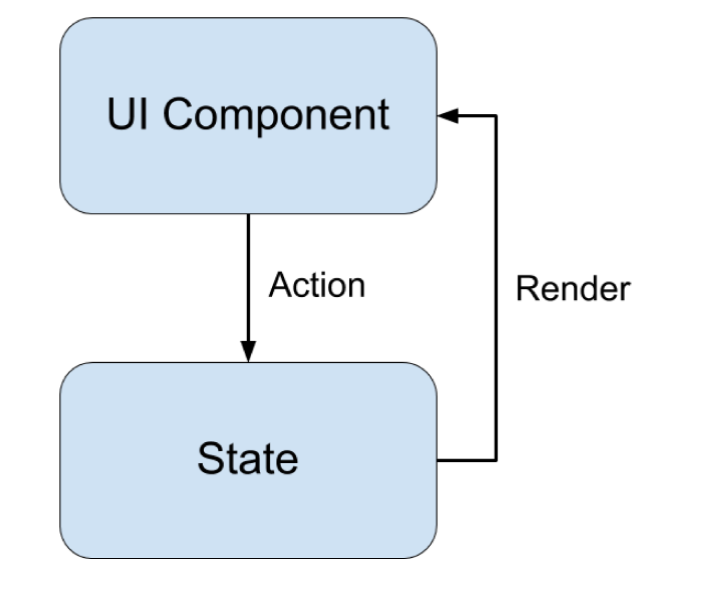
\includegraphics[height=5in]{reactArch.PNG}
	\caption{React Architechture}
	
\end{figure}

\subsubsection{Advantages over android studio}
It is cross-platform unlike android studio and can also be integrated with android studio java files.for those we include it in "node modules" directory in the project drectory.

\section{Android Studio AVD}
An Android Virtual Device (AVD) is a configuration that defines the characteristics of an Android phone, tablet, Wear OS, or Android TV device that you wantto simulate in the Android Emulator. The AVD Manager is an interface you can launch from Android Studio that helps you create and manage AVDs.

An AVD contains a hardware profile, system image, storage area, skin, and other properties.

\begin{figure}[!h]
	\centering
	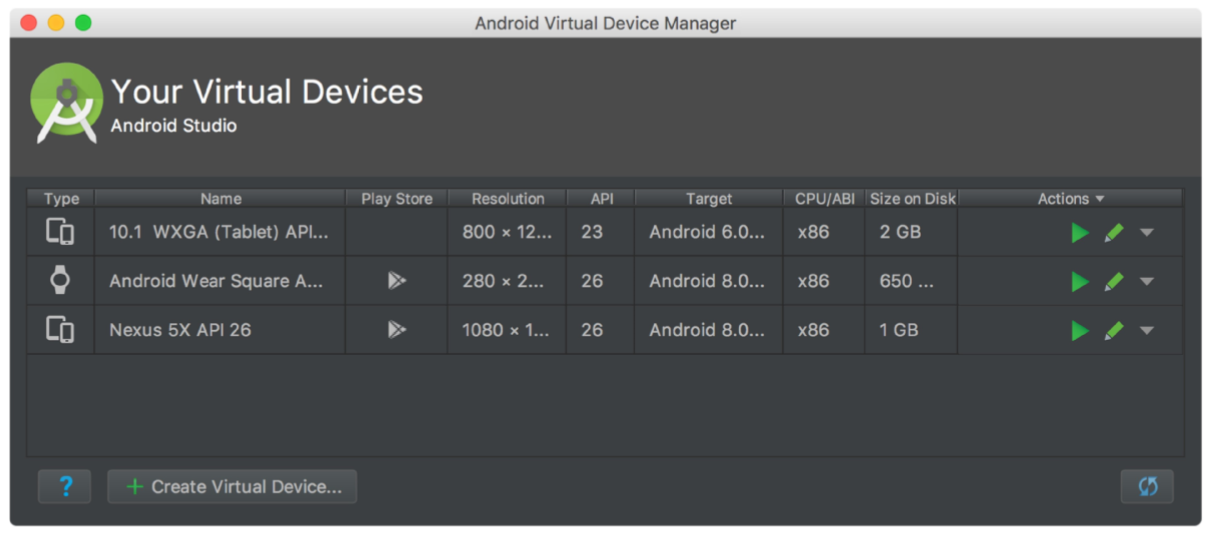
\includegraphics[height=3.1in]{avd.PNG}
	\caption{AVD manager in android studio}
	
\end{figure} 

\subsection{Hardware Profile}
The hardware profile defines the characteristics of a device as shipped from the factory. The AVD Manager comes preloaded with certain hardware profiles, such as Pixel devices, and you can define or customize the hardware profiles as needed.

\subsection{System Image}

We recommend that you create an AVD for each system image that your app could potentially support based on the user sdk setting in your manifest.


\subsection{Storage area}
The AVDhas a dedicated storage area on your development machine. It stores the device userdata, such as installed apps and settings, as well as an emulated SD card. If needed, you can use the AVD Manager to wipe user data, so the device has the same data asif it were new.

\subsection{Skin}
An emulator skin specifies the appearance of a device.Which also include the type of screen ratio your app is capable of supporting the best.


\subsection{Supportability}
AVD is supported only by the processors which support virtualization.

\section{Sublime Text}
Sublime Textis a proprietary cross-platform source code editor with a Python application program- ming interface (API). It natively supports many programming languages and markup languages, and functions can be added byusers with plugins, typically community-built and maintained under free- software licenses.\\
Stable release : 3.0 on 13 September 2017

\section{Firebase}
Firebase provides a realtime database and backend as a service. The service provides application de- velopers an APIthat allows application data to be synchronized across clients and stored on Firebase’s cloud.The company provides client libraries that enable integration with Android, iOS, JavaScript, Java, Objective-C, swift and Node.js applications. The database is also accessible through a REST API and bindings for several JavaScript frameworks such as AngularJS, React, Ember.js and Back- bone.js. The REST API uses the Server-Sent Events protocol, which is an API for creating HTTP connections for receiving push notifications from a server. Developers using the realtime database can secure their data by using the company’s server-side-enforced security rules.[20] Cloud Firestore whichis Firebase’s next generation of the Realtime Database was released for beta use.

\subsection{Properties :}
\subsubsection{Realtime}
Instead of typical HTTP requests, the Firebase Realtime Database uses data synchronization—every time data changes, any connected device receives that update within milliseconds.
\subsubsection{Offline}
Firebase apps remain responsive even when offline because the Firebase Realtime Database SDK persists your data to disk. Once connectivity is reestablished, the client device receives any changes it missed, synchronizing it with the current server state.

\subsection{Working}
The Firebase Realtime Database lets you build rich, collaborative applications by allowing secure access to the database directly from client-side code. Data is persisted locally, and even while offline, realtime events continue to fire, giving the end user a responsive experience. When the device regains connection, the Realtime Database synchronizes the local data changes with the remote updates that occurred while the client was offline, merging any conflicts automatically.
The Realtime Database provides a flexible, expression-based rules language, called Firebase Realtime Database Security Rules, to define how yourdata should be structured and when data can be read from or written to. When integrated with Firebase Authentication, developers can define who has access to what data, and how they can access it.
The Realtime Database is a NoSQL database and as such hasdifferent optimizations and functionality compared to a relational database. The Realtime Database APIis designed to only allow operations that can be executed quickly. This enables you to build a great realtime experience that can serve millions of users without compromising on responsiveness. Because ofthis, it is important to think about how users need to access your data and thenstructure it accordingly.

\subsubsection{Implementation}

1.Integrate the Firebase Realtime Database SDKs\\
Quickly include clients via Gradle, CocoaPods, or a script include.\\
\\
2.Create Realtime Database References\\
Reference your JSON data, such as ”users/user:1234/phoneNumber’” to set data or subscribe to data changes.\\
\\
3.Set Data and Listen for Changes\\
Use these references to write data or subscribe to changes.\\
\\
4.Enable Offline Persistence\\
Allow data to be written to the device’s local disk so it can be available while offline.\\
\\
5.Secure your data\\
Use Firebase Realtime Database Security Rules to secure your data.\\
\\


\newpage
\chapter{SOFTWARE REQUIREMENT SPECIFICATION}
\section{Introduction}
The requirements specification is a technical specification of requirements for the software products. It is the first step in the requirements analysis process it lists the requirements of a particular soft- ware system including functional, performance and security requirements. The requirements also provide usage scenarios from a user, an operational and an administrative perspective. The purpose of software requirements specification is to provide a detailed overview of the software project, its parameters and goals. This describes the project target audience and its user interface, hardware and software requirements.  It defines how the client, team and audience see the project andits functionality.


\section{Software requirements}
\begin{itemize}
	\item Android Device or Android emulator running android 6 (Android marshmallow) or latest
	\item Firebase (Databsae)
	\item React-native stable version (0.55)
	\item Sublime text or any other editor 
\end{itemize}
	
	
\section{Hardware reqirements}
\begin{itemize}
	\item intel i3 procrssor or above
	\item Clock speed 2GHz or above
	\item 4GB of ram
	\item Processor supporting virtualization
	\item connection to a network (if using an external device for debugging)
	
\end{itemize}
\newpage
\chapter{SYSTEM DESIGN}
\section{Flow chart}
\begin{figure}[!h]
	\centering
	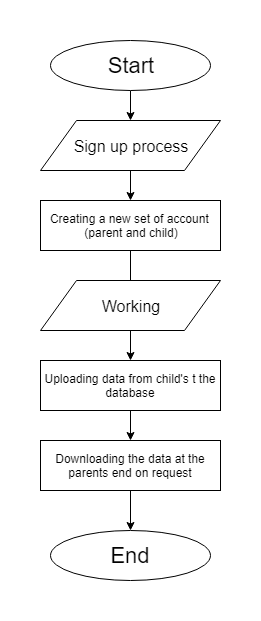
\includegraphics[height=7in]{flowchart.PNG}
	\caption{Flow chart}
\end{figure}

\section{Use case diagram}
\vspace{1in}
\begin{figure}[!h]
	\centering
	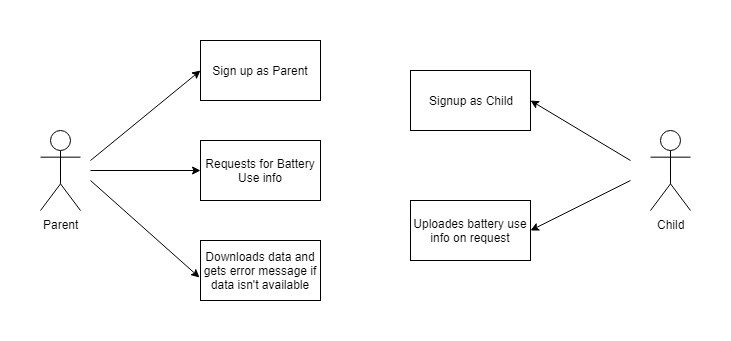
\includegraphics[height=3.4in]{UseCase.PNG}
	\caption{Use Case Diagram-}
\end{figure}
\newpage
\section{Activity Diagram}
\begin{figure}[!h]
	\centering
	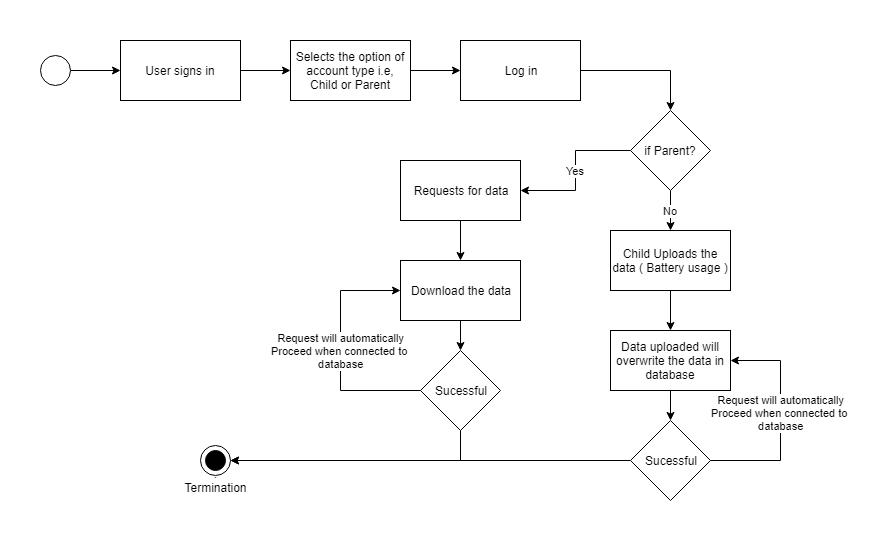
\includegraphics[height=4.5in]{Activity.PNG}
	\caption{Activity Diagram}
\end{figure}

\newpage
\chapter{IMPLEMENTATION}
\section{Introduction}
This project is basically a communication based application helpful of a family with busy guardians.It has a sign up functionality in which the new user can  sign up as “parent” or a “child” . the information regarding the usage of application of the child's phone will be uploaded and sent to database and then its been downloaded on the parent on request.

During the sign we ask for a “key” , it's nothing but a simple linking and deciding factor to bring together a set of parent and child. It helps establish a relationship between user, for example, a parent and its child will have a same key.
\begin{figure}[!h]
\centering
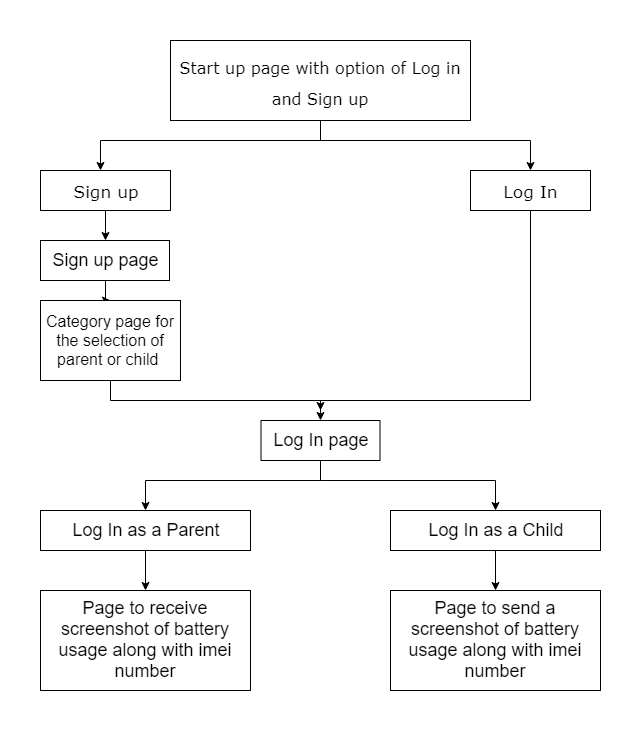
\includegraphics[height=5.3in]{flow.PNG}
\caption{Control flow in applicatition}
\end{figure}
\newpage
\section{Start up activity}
We will have two options here, If we sign up, it will direct us to sign up activity and then to category activity and further to login. Sign up activity helps us create and account (log in path) in the database and the we login after creation of account
\vspace{2cm}
\begin{figure}[!h]
	\centering
	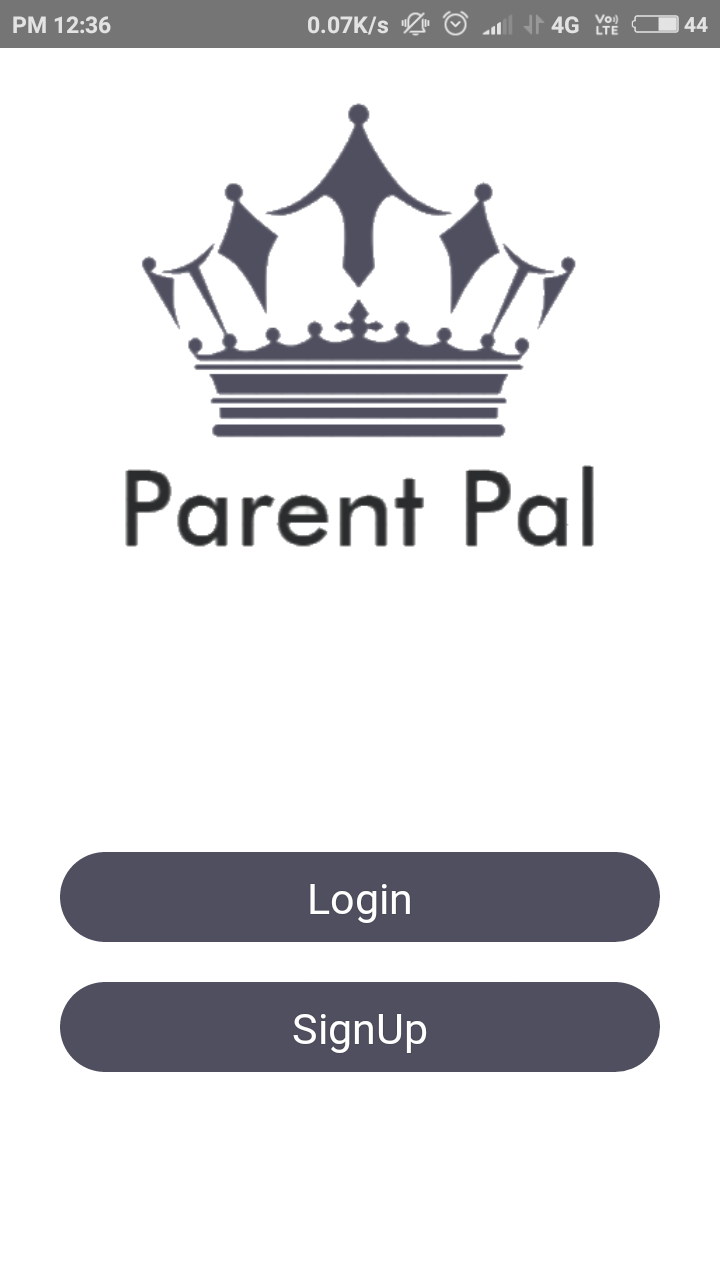
\includegraphics[height=7.3in]{Startup.PNG}
	\caption{Start up activity}
\end{figure}
\newpage

\section{Sign up sctivity}
Onclick of Sign up action button , it stores the value andredirects to another activity in which we select the type of account.
\begin{figure}[!h]
	\centering
	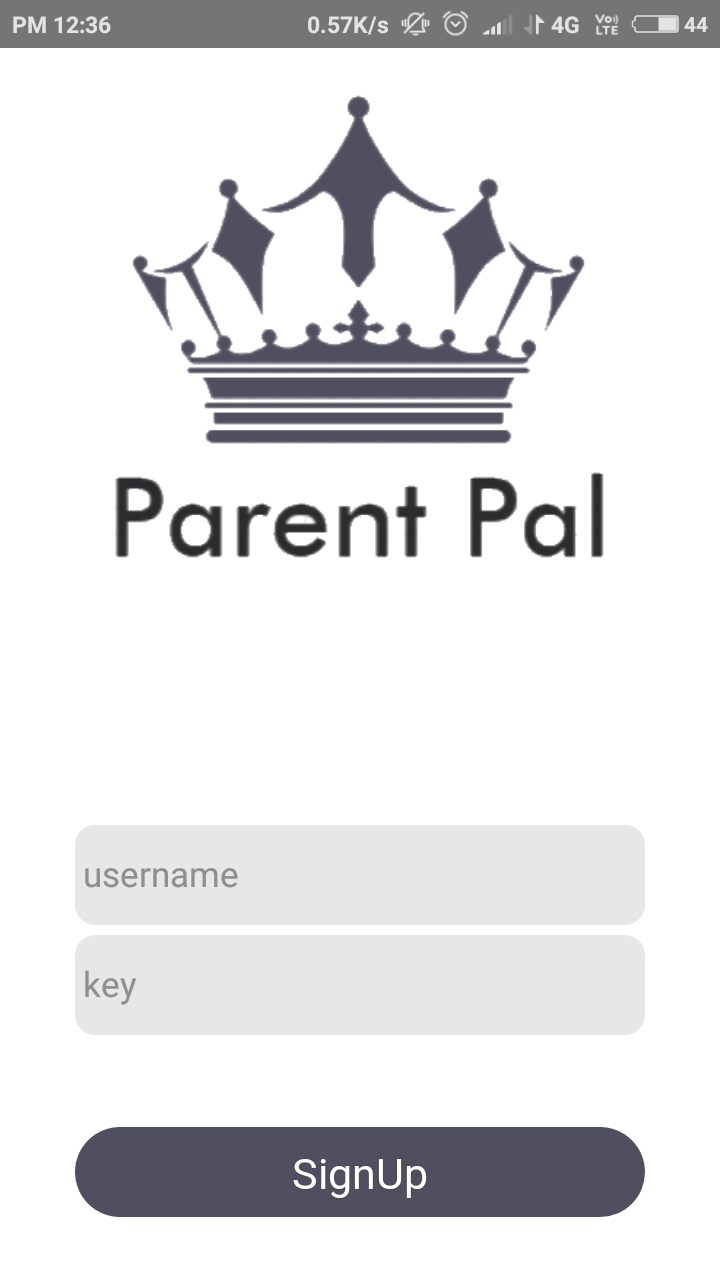
\includegraphics[height=7.3in]{Signup.PNG}
	\caption{Sign up activity}
\end{figure}
\newpage
\section{Log in activity}
On click of log in action button , it redirects according to the type of account.It redirect to a activity which allows us to upload data (if the account type is of child) or redirects to an activicy where can download the data (if the account type is or parent) .
\begin{figure}[!h]
	\centering
	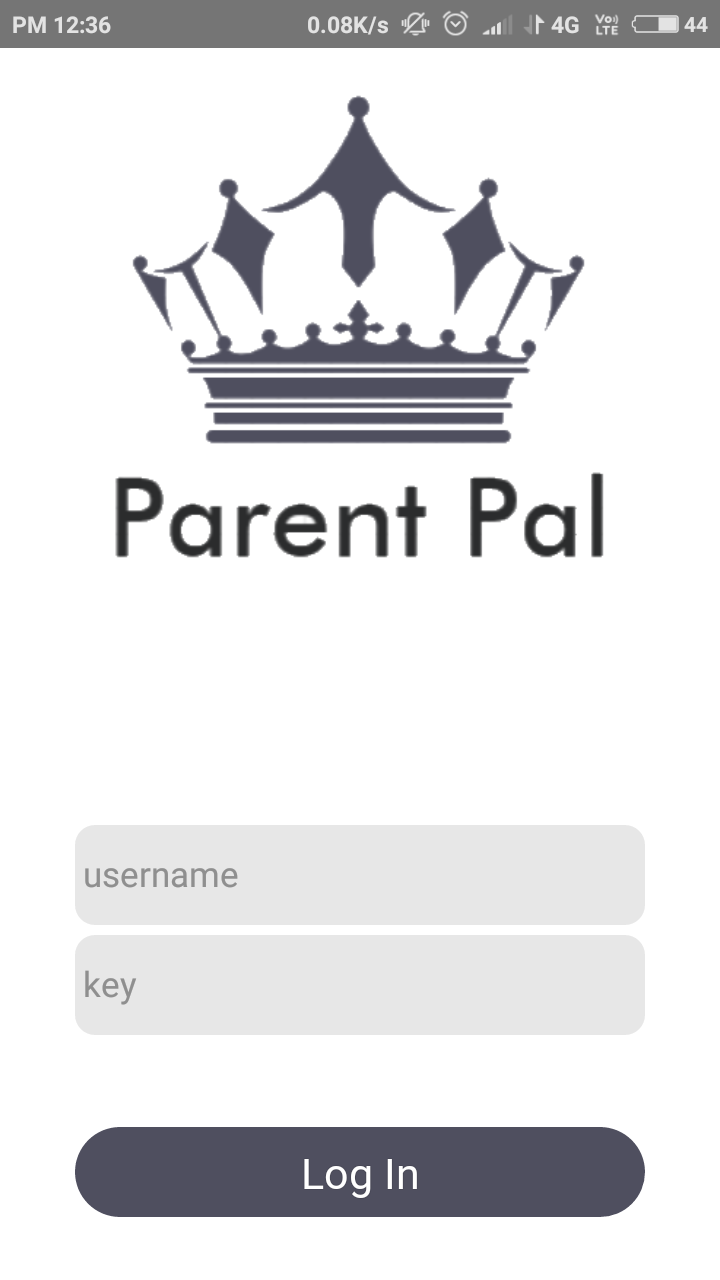
\includegraphics[height=7.3in]{Login.PNG}
	\caption{Log in activity}
\end{figure}
\newpage

\section{Category activity}
Helps us select the type of Account
\begin{figure}[!h]
	\centering
	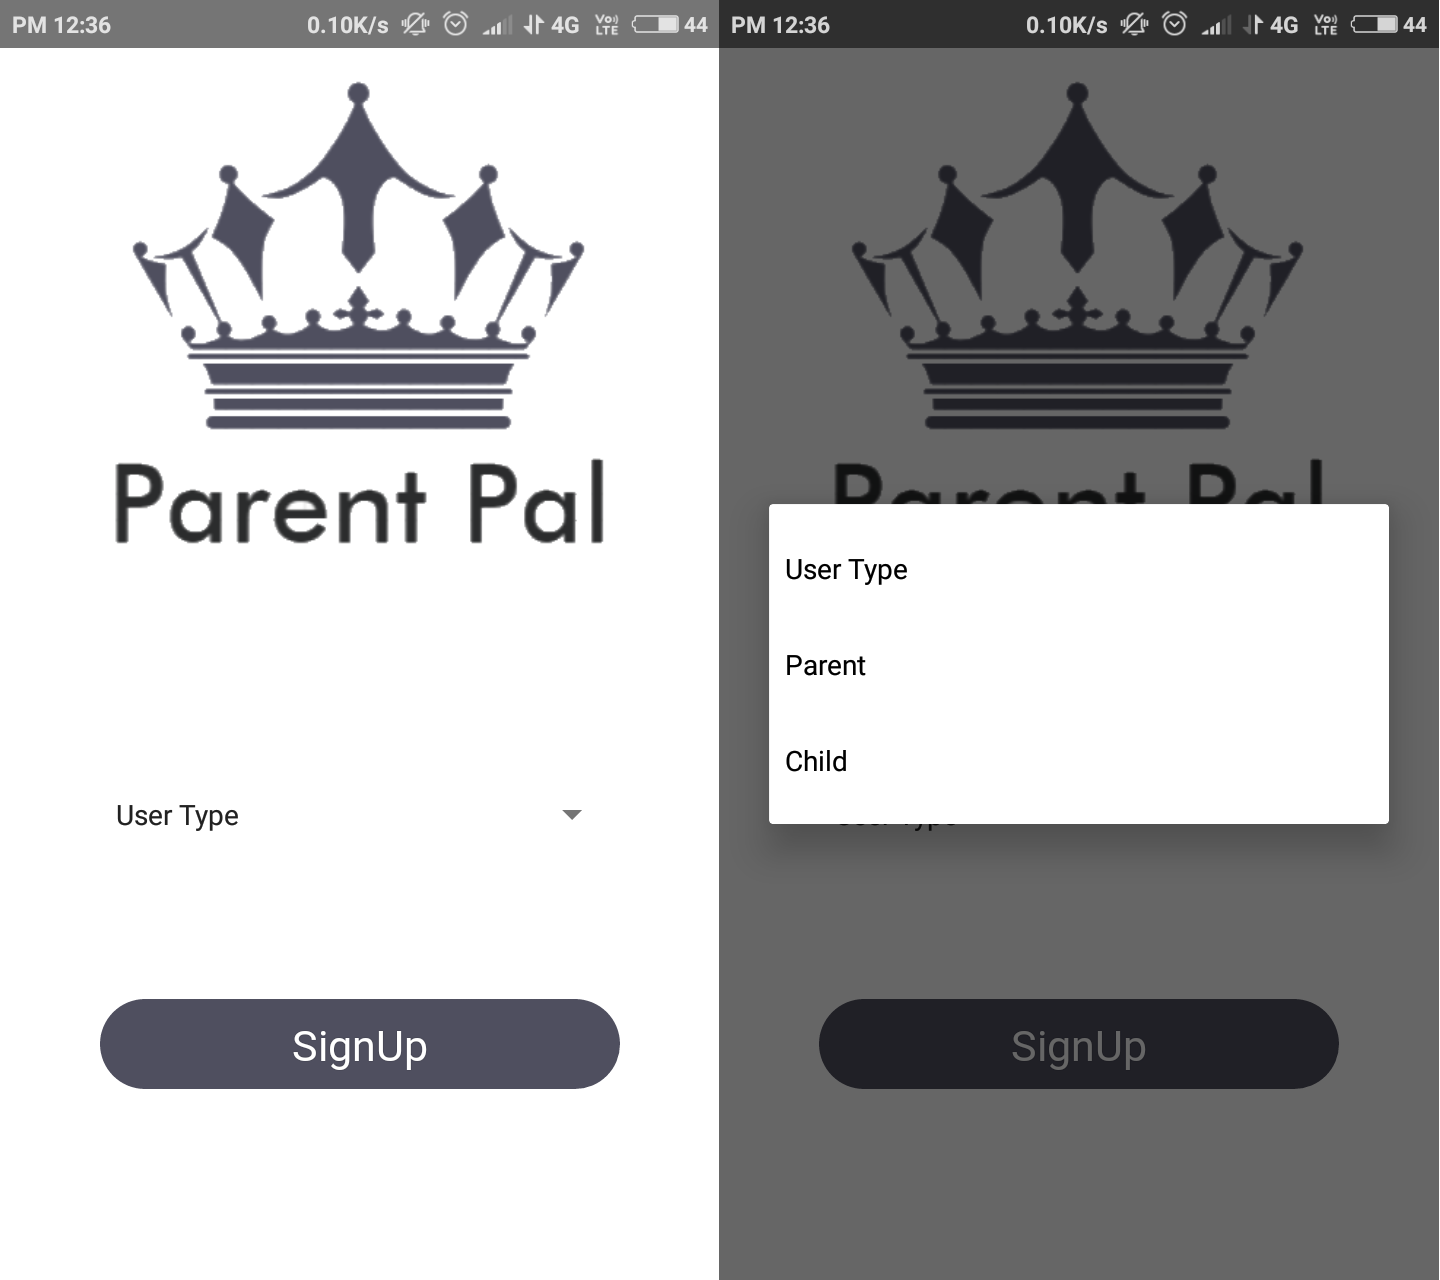
\includegraphics[height=6.3in]{catf.PNG}
	\caption{Category activity}
\end{figure}
\newpage
\section{Request activity}
For the reqest of uplaod or download
\begin{figure}[!h]
	\centering
	\includegraphics[height=7.3in]{Batuse.PNG}
	\caption{Request activity}
\end{figure}

\newpage
\chapter{RESULTS}
\section{Introduction}
Software testing is a critical element of software quality assurance and represents the ultimate review of specification, design and coding. In fact, testing is the one step in the software engineering process that could be viewed as destructive rather than constructive.
A strategy for software testing integrates software test case design methods into a well-planned series of steps that result in the successful construction of software. Testing is the set of activities that can be planned in advance and conducted systematically. The underlying motivation of program testing is to affirm software quality with methods that can economically and effectively apply to both strategic to both large and small-scale systems.

\section{Testing Objectives}
The main objective of performance testing is designed to test whether display is as expected and whether the webpage is functioning properly or not. 
As the test results are gathered and evaluated they begin to give a qualitative indication of the reliability of the code. If proper output is not obtained, the overall quality of the code is questioned. If, on the other hand, all the results which are not successful, are encountered, and are easily modifiable, then the following conclusion can be made: The tests are inadequate as the requirements mentioned are not compatible. The testing includes:
\begin{itemize}
	\item Checking whether the information is displayed or not.
	\item Checking whether all the players data is collected or not.
	\item Checking whether all the inputs are correctly taken or not.
	\item Verifying if all the pictures are displayed and none of the files are corrupted. 
\end{itemize}
\newpage

\section{Output screens}
Output is the battery use of the child's phone

\begin{figure}[!h]
\centering
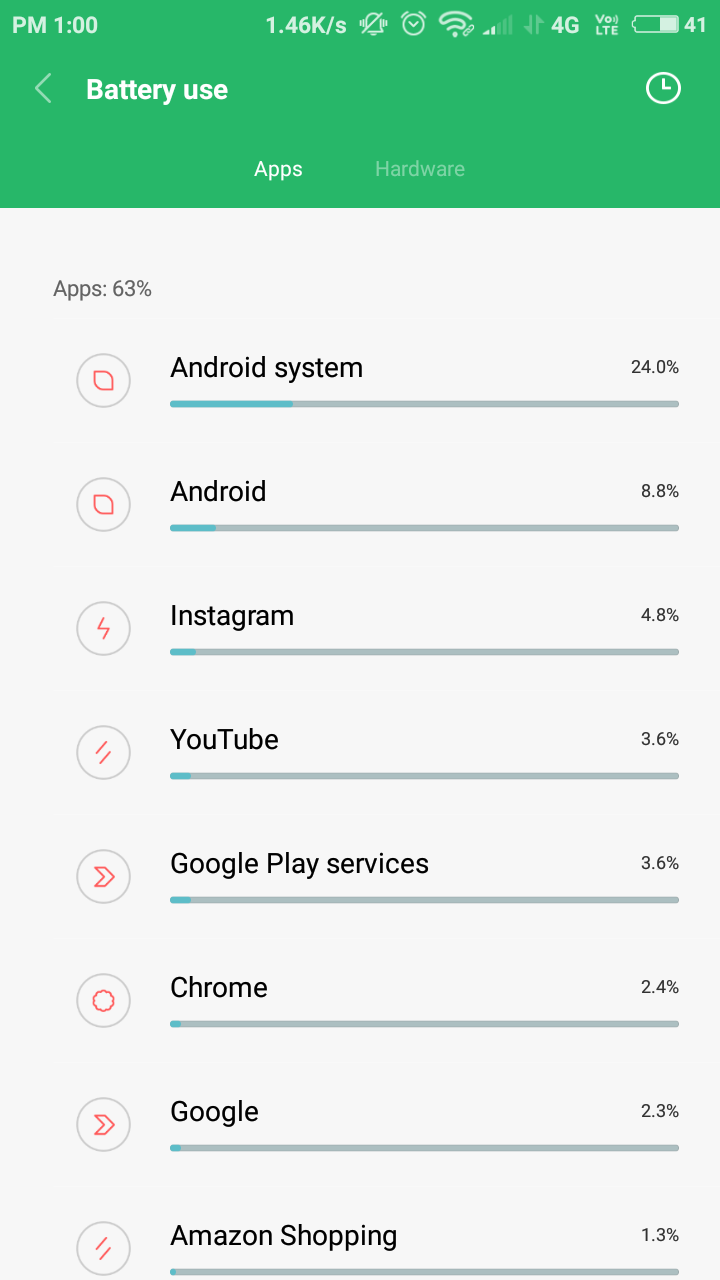
\includegraphics[height=7.5in]{out.PNG}
\caption{Output{\tiny }}
  
\end{figure}


\newpage


\chapter{CONCLUSION AND FUTURE SCOPE}

Overall we created an android (and ios) application using React-native which basically uploads and shares the battery use of a device. This was implemented on an android device and firebase.In future we will try to make it more advances by using live updates , background processes and remote control.This concept can also be used on other devices running on different platforms.



\newpage
\begin{thebibliography}{9}
\bibitem{react-native}
Text book
Mastering React Native by Eric Masiello 
\bibitem{bot}
RectJS tutorials
\\\texttt{https://www.tutorialspoint.com/reactjs/}

\bibitem{react-native}
React-native online documentataion and tutorials
\\\texttt{https://facebook.github.io/react-native/}
\bibitem{errors}
For debuggibg errors
\\\texttt{https://medium.com/}
\bibitem{bot}
For errors
\\\texttt{https://stackoverflow.com/}

\end{thebibliography}

















\end{document}
